%! TEX root = **/010-main.tex
% vim: spell spelllang=en:

\subsection{Na\"ive Bayes}%
\label{sub:naive-bayes}

% Think about hypothesis of independence of variables.  Do you have enough number of elements to obtain reliable probabilities?
% Keep that information for the discussion section.


Na\"ive Bayes works on the assumption of independence between variables in the dataset. First of all we checked weather or not this is a reasonable assumption in our dataset. To do so we calculated the correlation matrix, the farther apart the correlations are from 0 the more dependence there is between variables.

% Add correlation Matrix image

The correlations are much closer to 0 than expected. Therefore it isn't that farfetch to assume independence
between variables.

There are several types of Na\"ive Bayes algorithms:
    - Gaussian NB: Used when feature space is quantitative
    - Bernoulli NB: Used when feature space is Binary
    - Multinomial NB: Used when feature space is discrete counts

Our data is mostly numerical quantitative variables variables, therefore Gaussian Na\"ive Bayes will be applied from here on.

\subsection{Normalization}

First of all we executed the algorithm without performing any extra preprocessing of the data and obtained
relative poor results.

Confusion matrix on test set:
 [[208 200]
 [  3 189]]

Accuracy on test set:  0.6616666666666666


One of the problems we had when performing Na\"ive Bayes is that most of our data are continuous variables
which don't exactly follow a normal distribution. When using Gaussian Na\"ive Bayes will treat out data 
as if they followed such distribution. Therefore we tried different normalization techniques to make our
data more Gaussian-like

\subsection{Standardization}

After standardizing out data, std=1, mean=0. We executed the algorithm again and found better results:

Confusion matrix on test set:
 [[287 121]
 [  2 190]]

Accuracy on test set:  0.795

\subsection{Power Transforms}

Power transforms is a preprocessing algorithm that simply explained aims to make our data more Gaussian-like. We executed Gaussian Na\"ive Bayes and found by far the best results:

Confusion matrix on test set:
 [[357  51]
 [ 19 173]]

Accuracy on test set:  0.8833333333333333

We find it quite surprising to see how different normalization techniques yield such different final accuracy results. We decided to continue forward with the Power Transformed data as it had over 0.1
more accuracy that the rest.

\subsection{Parameter tuning}

Na\"ive Bayes doesn't have many hyperparameters, in fact we will only analyse \texttt{var\_smoothing} which determines the amount Laplace smoothing applied.

\begin{figure}[H]
    \centering
    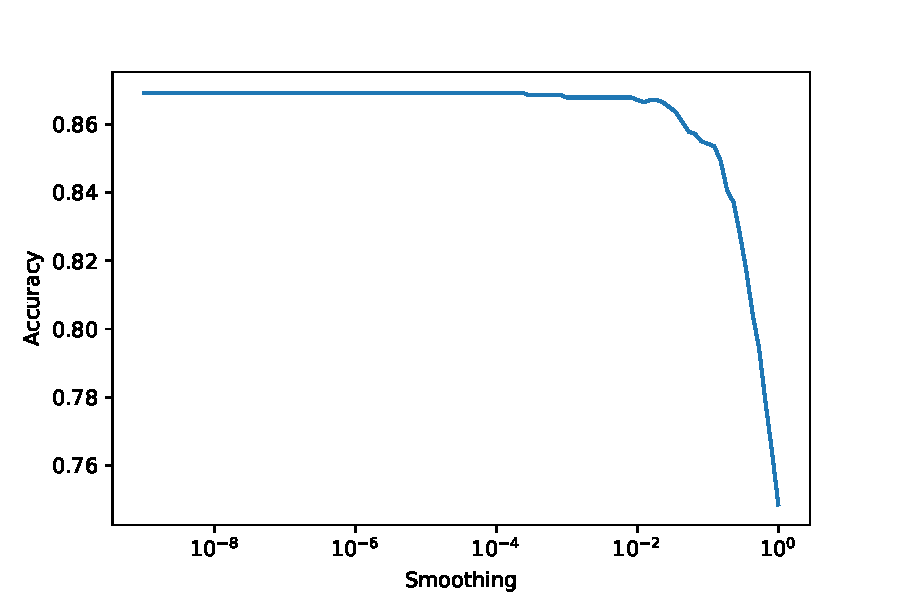
\includegraphics{figures/naive_bayes_smoothing_cv.pdf}
    \caption{Na\"ive Bayes smoothing}%
    \label{fig:naive_bayes_smoothing_cv}
\end{figure}

Looking at the image we can see that the accuracy barely changes when the \texttt{var\_smoothing} is in the range $[10^{-9}, 10^{-2}]$. Therefore its better to leave the default $10^{-9}$.
